\documentclass{article}
\usepackage{amsmath}
\usepackage{amssymb}
\usepackage{enumerate}
\usepackage{graphicx}

\title{MAT -- 112: Calculus I and Modeling\\
\large{Solution 9}}
\author{Thomas R. Cameron}
\date{4/27/2018}

\begin{document}
\maketitle

\subsection*{Other Problems}

\paragraph*{Problem 1.} Consider the differential equation
\[
\frac{dy}{dt}=f(t,y),~\quad~y(t_{0})=y_{0}.
\]
We are interested in approximating this differential equation with a step size of $h$. Therefore, the next point $(t_{1},y_{1})$ satisfies $t_{1}=t_{0}+h$ and
\begin{align*}
y_{1}-y_{0} &= \int_{y_{0}}^{y_{1}}dy~\text{(by the F.T.C.)} \\
&= \int_{t_{0}}^{t_{1}}f(t,y)dt~\text{(since $dy=f(t,y)dt$).}
\end{align*}
It follows that we can approximate the next $y$-value ($y_{1}$) by using numerical integration techniques. If we employ the left-hand rule, then we have
\[
y_{1}\approx y_{0}+hf(t_{0},y_{0}).
\]
This is Euler's method. If we use the trapezoidal method to approximate the integral, then we have
\[
y_{1}\approx y_{0}+\frac{h}{2}\left(f(t_{0},y_{0})+f(t_{1},y_{1})\right).
\]
The problem here is that we have $y_{1}$ on both sides of the equation. For this reason, we employ Euler's method to approximate $y_{1}$ on the right hand side of the equation. Thus, we have
\[
y_{1}\approx y_{0}+\frac{h}{2}\left(f(t_{0},y_{0})+f(t_{0}+h,y_{0}+hf(t_{0},y_{0}))\right).
\]
This is what we called the \emph{Trapezoidal method}. In practice,  this is referred to as one of the many multi-step methods. Perhaps the most famous multi-step method is the Runge-Kutta method, which can be derived from Simpson's rule. 

\newpage

\paragraph*{Problem 2.} See the figures below. 

\begin{figure}[h!]
\centering
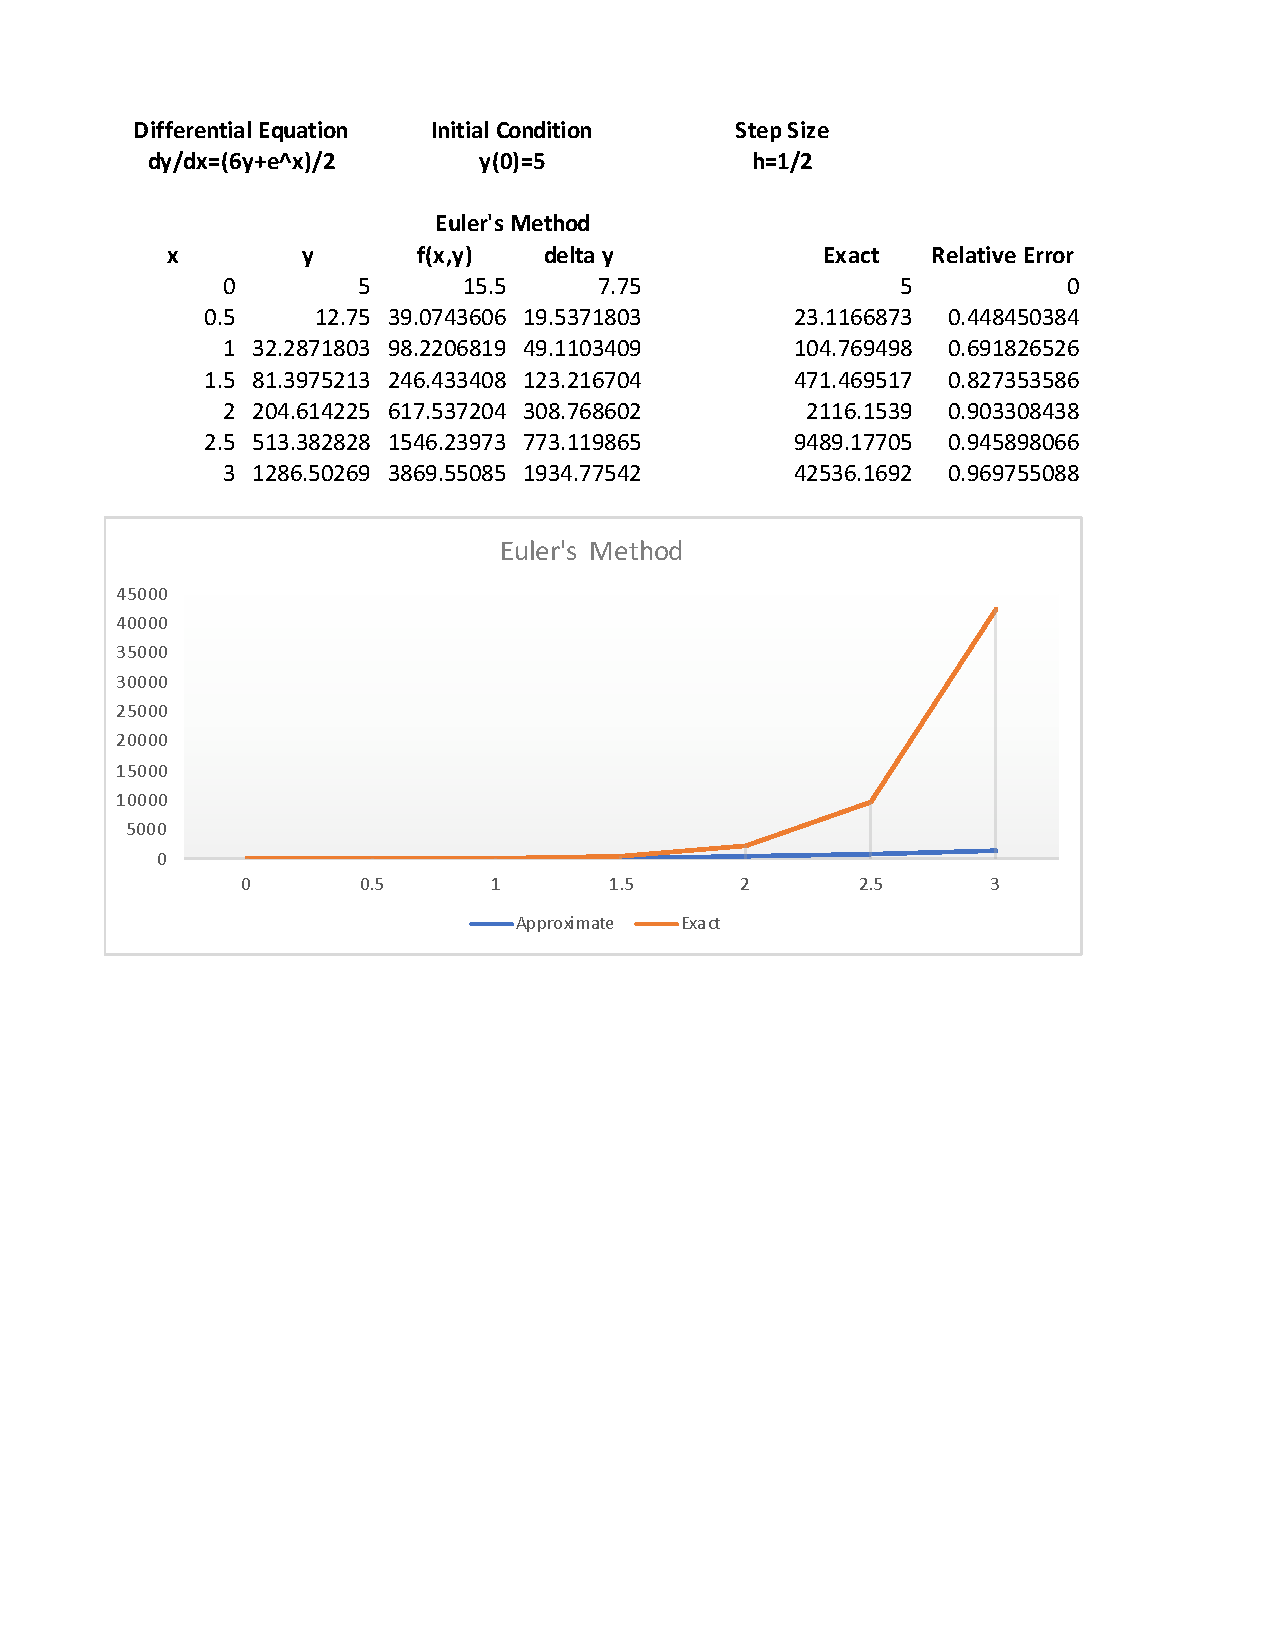
\includegraphics[trim={0 11cm 0 0},clip,scale=0.5]{hw9_fig1}
\end{figure}

\begin{figure}[h!]
\centering
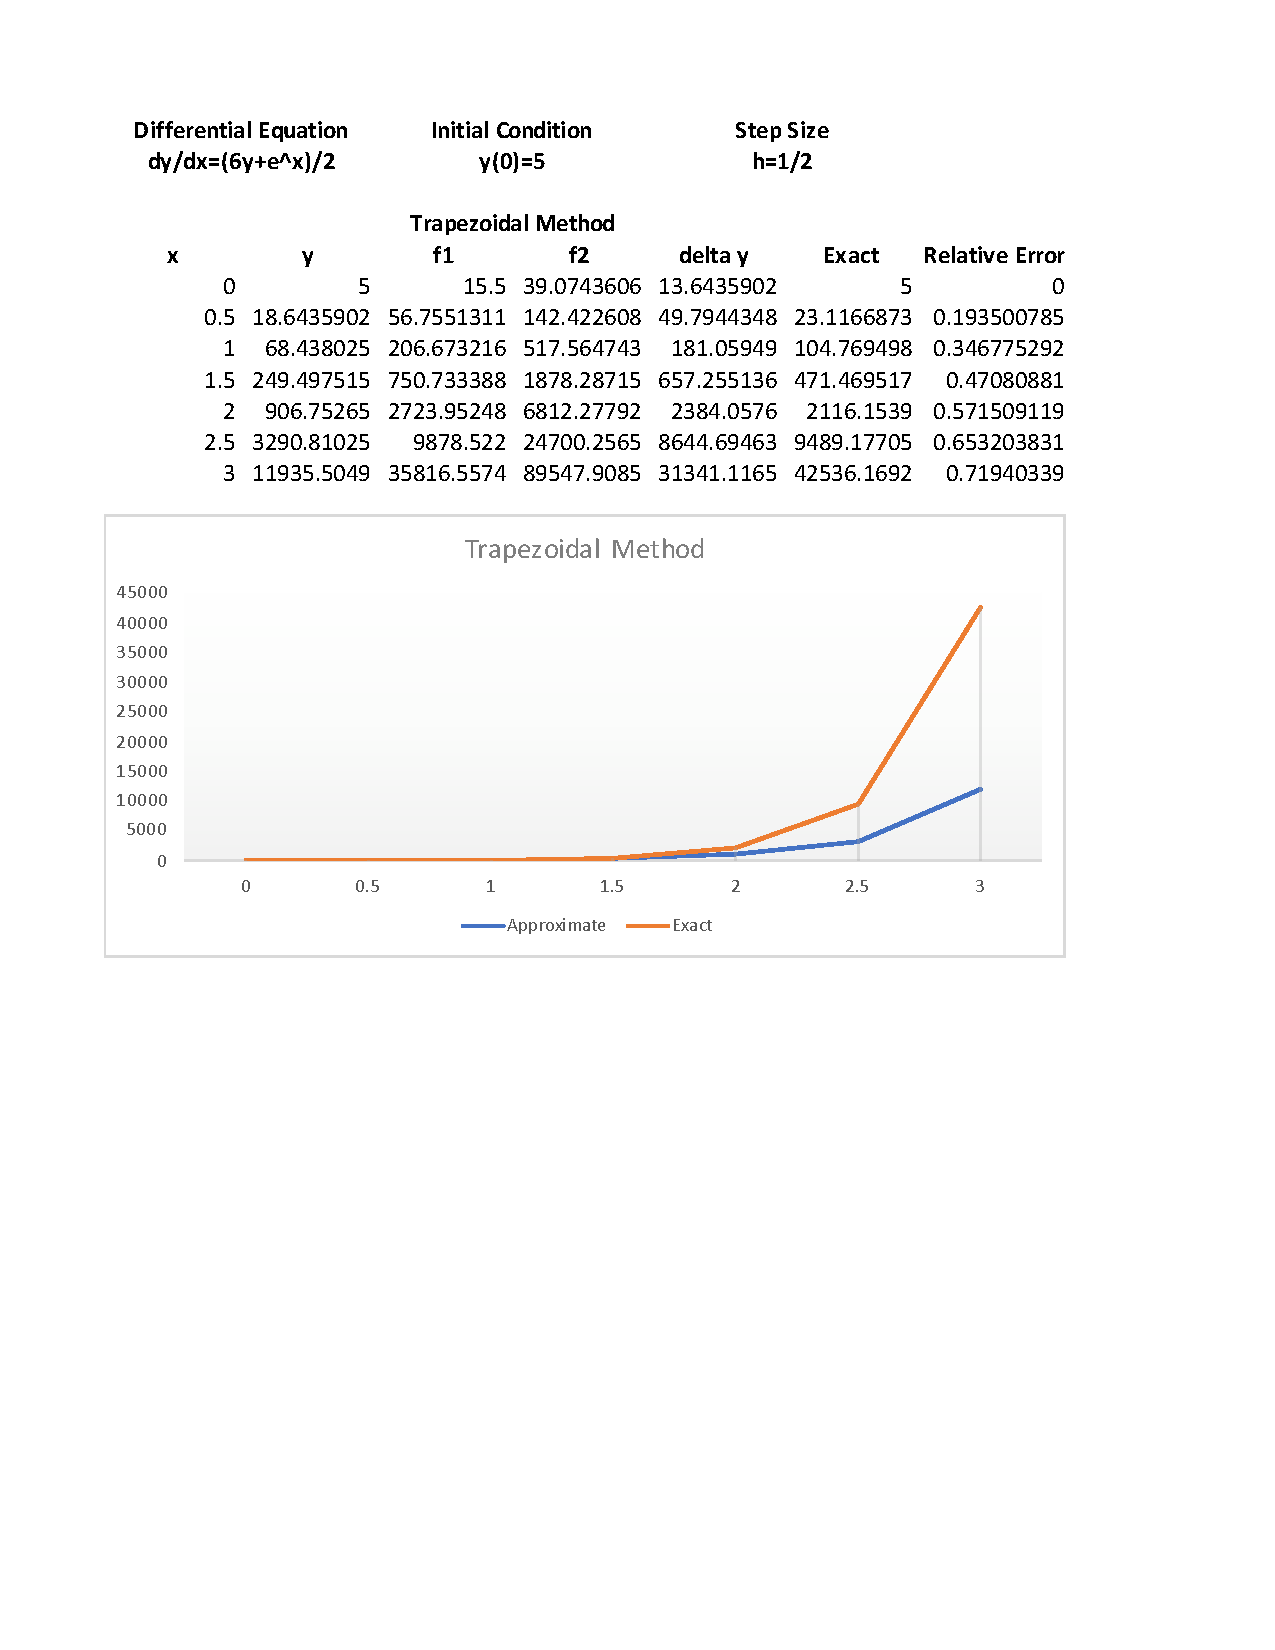
\includegraphics[trim={0 11cm 0 0},clip,scale=0.5]{hw9_fig2}
\end{figure}

\end{document}